\documentclass[tikz,border=2pt]{standalone}
\usepackage{amsmath}
\usepackage{amssymb}
\usepackage{xcolor}

\definecolor{journalink}{HTML}{1F1C18}
\definecolor{journalmuted}{HTML}{8A7F72}
\definecolor{journalaccent}{HTML}{9C2D2D}

\newcommand{\axisrow}[2]{%
  \draw[journalink, line width=0.8pt, ->, >=stealth] (0,#1) -- (5.8,#1);
  \node[journalink, right] at (5.8,#1) {#2};
  \draw[journalink, line width=0.8pt] (1.2,{#1+0.16}) -- (1.2,{#1-0.16});
  \node[journalink, below, font=\small] at (1.2,{#1-0.16}) {$0$};
  \draw[journalink, line width=0.8pt] (3.0,{#1+0.16}) -- (3.0,{#1-0.16});
  \node[journalink, below, font=\small] at (3.0,{#1-0.16}) {$1$};
  \draw[journalink, line width=0.8pt] (4.8,{#1+0.16}) -- (4.8,{#1-0.16});
  \node[journalink, below, font=\small] at (4.8,{#1-0.16}) {$2$};
}
\newcommand{\segrow}[3]{\draw[journalaccent, line width=1.8pt] (#2,#1) -- (#3,#1);}
\newcommand{\closeddot}[2]{\fill[journalink] (#2,#1) circle (2.2pt);}
\newcommand{\opendot}[2]{\draw[journalink, line width=1.0pt, fill=white] (#2,#1) circle (2.2pt);}

\begin{document}
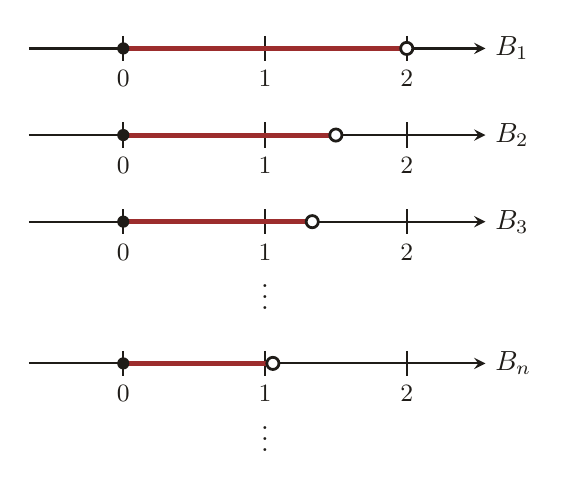
\begin{tikzpicture}[x=1cm, y=1cm, every node/.style={font=\normalsize}]

  \axisrow{0}{$B_1$}
  \segrow{0}{1.2}{4.8}
  \closeddot{0}{1.2}
  \opendot{0}{4.8}

  \axisrow{-1.1}{$B_2$}
  \segrow{-1.1}{1.2}{3.9}
  \closeddot{-1.1}{1.2}
  \opendot{-1.1}{3.9}

  \axisrow{-2.2}{$B_3$}
  \segrow{-2.2}{1.2}{3.6}
  \closeddot{-2.2}{1.2}
  \opendot{-2.2}{3.6}

  \node[journalink] at (3.0,-3.05) {$\vdots$};

  \axisrow{-4.0}{$B_n$}
  \segrow{-4.0}{1.2}{3.1}
  \closeddot{-4.0}{1.2}
  \opendot{-4.0}{3.1}

  \node[journalink] at (3.0,-4.85) {$\vdots$};

\end{tikzpicture}
\end{document}
